\documentclass[12pt, titlepage]{article}

\usepackage{booktabs}
\usepackage{tabularx}
\usepackage{hyperref}
\usepackage{graphicx}
\usepackage{float}



\hypersetup{
    colorlinks,
    citecolor=black,
    filecolor=black,
    linkcolor=red,
    urlcolor=blue
}
\usepackage[round]{natbib}

\title{SE 3XA3: Software Requirements Specification\\AAA Tetris}

\author{Team \#115, AAA Solutions
		\\ Abdallah Taha and tahaa8
		\\ Ali Tabar and sahraeia
		\\ Andrew Carvalino and carvalia
}

\date{\today}

\begin{document}

\maketitle

\pagenumbering{roman}
\tableofcontents
\listoftables
\listoffigures

\begin{table}[bp]
\caption{\bf Revision History}
\begin{tabularx}{\textwidth}{p{3cm}p{2cm}X}
\toprule {\bf Date} & {\bf Version} & {\bf Notes}\\
\midrule
Feb 10, 2021 & 1.0 & Sections 2.1, 2.2, 2.3 added\\
Feb 12, 2021 & 1.1 & Sections 2 and 3 completed\\
Feb 12, 2021 & 1.2 & Section 1 completed\\
\bottomrule
\end{tabularx}
\end{table}

\newpage

\pagenumbering{arabic}

This document describes the requirements for AAA Tetris The template for the Software
Requirements Specification (SRS) is a subset of the Volere
template~\citep{RobertsonAndRobertson2012}.

\section{Project Drivers}

\subsection{The Purpose of the Project}
The purpose of this project is to create a Tetris game based on an initial version of it found on GitHub, but with major improvements. First of all, the original game is just a single Python file, which can only be launched via executing a console command. Our version of the game will be on a web browser page, which will immediately be launched upon opening the page. Additionally, we will be adding on several features. One such feature will be an adjustable difficulty feature which the user can use to make the game either easier or harder. Another feature added to the game will be levels and / or different game modes - this will give the user some incentive to keep playing the game, and add some variety to the experience. 
One improvement made on the game will be to improve its visuals - overall, making the game’s UI look more appealing to anyone playing.

\subsection{The Stakeholders}

\subsubsection{The Client}
The client of this project would be the company who is releasing the game for us. They will review the game before its release to the public, and ensure they are happy with the product. The game will be released under their name.
\subsubsection{The Customers}

The customer of the project will be anyone in the general public who is interested in playing the game. It is expected that they all have a computer with access to a web browser and an internet connection, enabling them to run and play the game. Additionally, they should have access to a keyboard and monitor to be able to input controls into the game, and see the game on their screen.

\subsubsection{Other Stakeholders}

The Developers:\\
The developers of this project are the members of AAA Solutions. Our job is to develop a Tetris game, using the original version found on GitHub as a reference. Throughout the developing process, we will test the game and change or improve the design as we see fit.

\subsection{Mandated Constraints}

This section of the template has been modified from the original to include the subsections of 1.3.1 to 1.3.7.

\subsubsection{Solution Constraints}
The game should be able to run on all popular desktop browsers (Google Chrome, Microsoft Edge, Mozilla FireFox) which support JavaScript. This project will only cover game support for playing on computers, as the controls will be inputted via keyboard. It is assumed that the general public will use popular web browsers, removing the need for optimizing the game to run on outdated or obscure web browsers.

\subsubsection{Implementation Environment of the Current System}
\begin{figure}[H]
\caption{Implementation Environment}
\centering
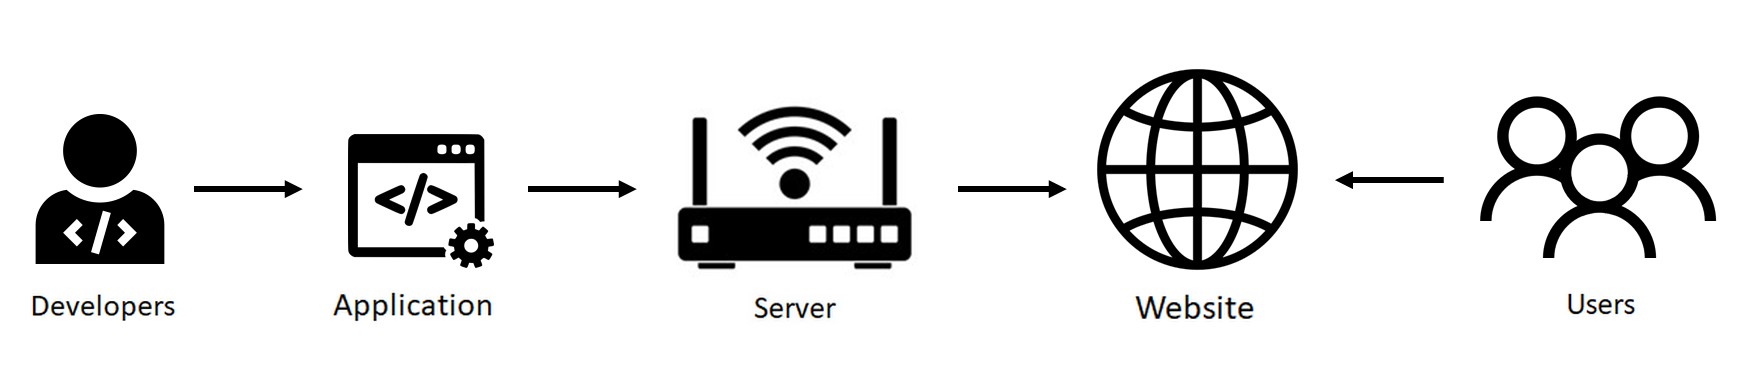
\includegraphics[width=0.95\linewidth]{environment.png}
\end{figure}

\subsubsection{Partner or Collaborative Applications}
The game does not have any partner or collaborative applications - however, it does rely on popular web browsers being able to run JavaScript and continuing support for it. This is not a very big concern, as HTML is the standard language for web pages, and JavaScript is what is used to interact with those web pages - so the game should have continued support for a very long time. If published on an online website for anyone to access via the internet, the product will rely on having some sort of domain hosting service.

\subsubsection{Anticipated Workplace Environment}
There is no specific anticipated workplace environment for this product. Ideally, it can be played anywhere, at any time, as long as the user is using a desktop PC or laptop with an internet connection.

\subsubsection{Schedule Constraints}

We have scheduled the project to be fully finished by the week of April 5th.
\subsubsection{Budget Constraints}
We do not currently have any sort of budget constraints for this project. All tools and resources necessary to work on the project are open-source, with no money necessary. Should a situation arise where a resource is required for the completion of the project, the cost will be covered out of pocket from the developers.

\subsubsection{Enterprise Constraints}

The finished product will be available for anyone - free access to play the game will be available to the entirety of the public.

\subsection{Naming Conventions and Terminology}

\subsubsection{Definitions of All Terms, Including Acronyms, Used by Stakeholders Involved in the Project}
\begin{table}[H]
\caption{\bf Definitions}
\begin{center}
\begin{tabular}{|c|c|}
\hline
ACRONYM/ABBREVIATION & INTENDED MEANING\\
\hline
AAAS & AAA Solutions\\
\hline
JS & JavaScript\\
\hline
HTML &Hypertext Markup Language\\
\hline
UI & User Interface\\
\hline
GUI & Grahical User Interface\\
\hline
Ex & Example\\
\hline
OS & Operating System\\
\hline
Etc & Et Cetera\\
\hline
Wi-Fi & Wireless Fidelity\\
\hline
IDE & Integrated Development Environment\\
\hline
GL & Gitlab\\
\hline
Product & The game being developed, in its finished state\\
\hline
Project & The development of the game, in an unfinished state\\
\hline
Client & The person(s) the product is made for\\
\hline
Customer & The person(s) that will use the finished product\\
\hline
The program & The coding that makes up the game\\
\hline
\end{tabular}
\end{center}
\label{default}
\end{table}%





\subsection{Relevant Facts and Assumptions}

\subsubsection{Relevant Facts}

We have a few business rules for our team.
The first rule is that we all reserve the right to question each other and ask for further explanations when viewing parts of the project that other team members have worked on. The reason for this is that as a team, we all deserve to know the reasoning behind other team members’ decisions and how our parts will function in conjunction with theirs.
The second rule is that the entire team will have a group meeting at least two hours before a project deliverable is due. This will ensure for adequate time for the team to check over the deliverable together, sort out any discrepancies, and correct errors.

\subsubsection{Assumptions}
The developers are assuming that all software being used in the creation of the project will be free, open source software. This will include coding IDEs and software packages such as JavaScript or Python libraries. 

\section{Functional Requirements}

\subsection{The Scope of the Work and the Product}

\subsubsection{The Context of the Work}
\begin{figure}[H]
\caption{Work Context}
\centering
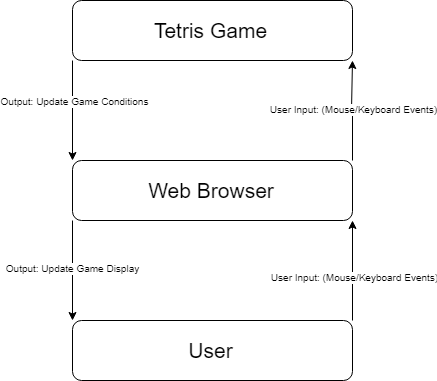
\includegraphics[width=0.95\linewidth]{Context.png}
\end{figure}


\subsubsection*{Work Partitioning}
\begin{table}[H]
\caption{Work Partitioning Part I}
\hskip-2.5cm\begin{tabular}{|c|c|c|c|}
\hline
Event Number & Event Name & Input & Output\\
\hline
1 & Tetris game Creation & Developer code & Web Browser\\
\hline
2 & Tetris game Audio & Microphone & Audio output device\\
\hline
3 & Tetris Full Row of Blocks & Developer graphics and code & Web Browser\\
\hline
4 & Blocks Overflow Outside of Grid & Developer code & Web Browser\\
\hline
5 & Tetris Score Calculation & Developer code & Web Browser\\
\hline
6 & Tetris Game Final Revision & Developer code & Web Browser\\
\hline
\end{tabular}
\label{default}
\end{table}%

\begin{table}[H]
\caption{Work Partitioning Part II}
\hskip-2.5cm\begin{tabular}{|c|c|}

\hline
Event Number & Summary of BUC\\
\hline
1 & Recreate a terminal based game that works on multiple web browsers\\ 
\hline
2 & Record sound effect to be displayed in the game\\
\hline
3 & Create different functions to perform the game mechanics in this project\\
\hline
4 & Create overflow detection when blocks fall outside of grid then display an end screen\\
\hline
5 & Create a detection system for when row is full and calculate current score\\
\hline
6 & Finishing edits to the project\\
\hline

\end{tabular}
\label{default}
\end{table}%


    
    
\subsubsection{Individual Product Use Cases}

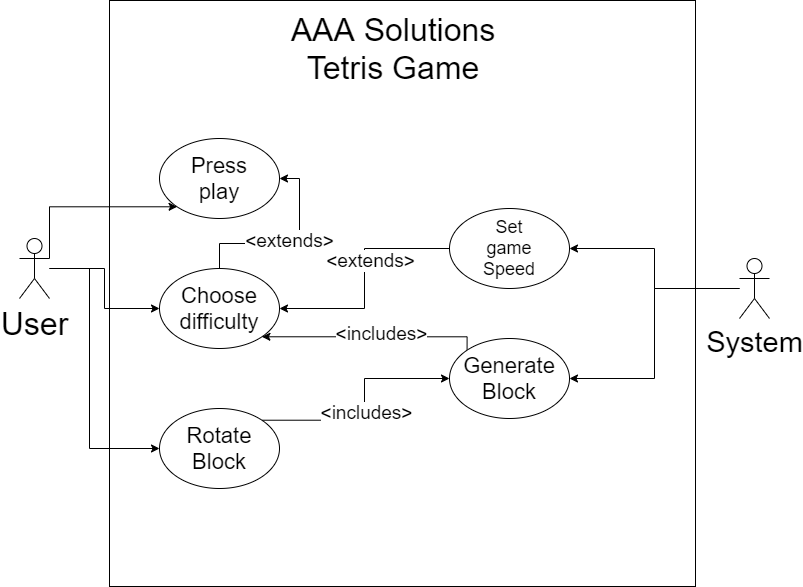
\includegraphics[width=0.95\linewidth]{usecasexa3.png}

\subsection{Functional Requirements}
\begin{itemize}
    \item
    Executable HTML file will launch in a new web browser window.    \subitem
    Fit Criterion or Test Case: \\
    Check if a new tab opens within the web browser when aforementioned HTML file is executed.    
    \item
    The HTML will be executable by any browser with JavaScript compatibility.    \subitem
    Fit Criterion or Test Case: \\
    Execute the HTML file with different major browsers and check if it executes properly.    
    \item
    Initial condition of the game will display a start menu and stay in a standby sate until it receives user input.    \subitem
    Fit Criterion or Test Case: \\
    Check that the game stays in the start menu when executed until it receives an input.    
    \item
    When the game starts the game state will have zero blocks within the grid and score will be set to zero.    \subitem
    Fit Criterion or Test Case: \\
    Check the display of the grid and scoreboard when starting the game to check if the score is at 0 and no blocks are in the grid.    
    \item
    Blocks will start flowing one by one onto the grid and will rotate based upon user input when the user pushes the play game button.    \subitem
    Fit Criterion or Test Case: \\
    Let user press play on the game and check that the blocks begin flowing onto grid one by one and input the WASD keys to check for the 90-degree rotation.    
    \item
    During the game if a block lands outside of the grid of the game then the game will terminate and display final score to the user.    \subitem
    Fit Criterion or Test Case: \\
    Check that the game returns the users final score and displays the game over screen.    
    \end{itemize}
    



\section{Non-functional Requirements}

\subsection{Look and Feel Requirements}
\subsubsection{Appearance Requirements}
\begin{itemize}
\item The user interface shall be well formatted and separated based on score and game grid.
\item The user interface will include the company logo.
\item The user interface will have different colors for different shaped blocks
\item The user interface will have a distinguished game grid section and separate current score section
\end{itemize}
\subsubsection{Style Requirements}
\begin{itemize}
    \item The user interface will have a consistent font throughout
    \item Blocks will generate and fall seamlessly onto the game grid
    \item Buttons should be easily identified and responsive 
\end{itemize}

\subsection{Usability and Humanity Requirements}
\subsubsection{Ease of Use Requirements}
The game shall be playable by any user with basic understanding of navigating a web browser.
\subsubsection{Personalization and Internationalization Requirements}
N/A
\subsubsection{Learning Requirements}
A user shall be able to fully understand the game within five minutes of executing the program.
\subsubsection{Understandability and Politeness Requirements }
The system shall use text to indicate that an action can be performed and shall only use icons when the icon is commonly associated with a standard action (i.e trashcan icon for delete).
\subsubsection{Accessibility Requirements}
This game will be playable to any user that can operate a mouse and keyboard and has access to a web browser.
\subsubsection{Convenience Requirements}
Game will automatically display the play again button for the user when the game ends.


\subsection{Performance Requirements}
\subsubsection{Speed and Latency Requirements}
System shall take no longer then 5 seconds to set up the game once the play button has been pressed. System shall also display the game over menu and calculate the final score in under 3 seconds of game ending.
\subsubsection{Safety-Critical Requirements}
N/A
\subsubsection{Precision or Accuracy Requirements}
Score shall have zero decimal points and will always be a whole number. Game block will only rotate by 90 degrees and block shall only move one grid box horizontally upon user input.
\subsubsection{Reliability and Availability Requirements}
System shall go down for no longer then 24 hours every 2 years.
\subsubsection{Robustness or Fault-Tolerance Requirements}
N/A
\subsubsection{Capacity Requirements}
System shall only record previous games score and the current highscore.
\subsubsection{Scalability or Extensibility Requirements}
N/A
\subsubsection{Longevity Requirements}
Expected lifetime of the system shall be indefinite.

\subsection{Operational and Environmental Requirements}
\subsubsection{Expected Physical Environment}
This application shall run on any device with a web browser and a internet connection.
\subsubsection{Wider Environment Requirements}
N/A
\subsubsection{Requirements for Interfacing with Adjacent Systems}
N/A
\subsubsection{Productization Requirements}
N/A
\subsubsection{Release Requirements}
Yearly software releases will be deployed to maintain and improve the application based on client demands and needs.

\subsection{Maintainability and Support Requirements}
\subsubsection{Maintenance Requirements}
Maintenance should only take one day requiring the application to only be down one day at a time.
\subsubsection{Supportability Requirements}
Product should ensure that any device running a web browser should have capability to run the game.
\subsubsection{Adaptability Requirements}
N/A

\subsection{Security Requirements}
\subsubsection{Access Requirements}
Any user can have access to the UI of the product given they have a internet connection and a web browser. Only developers will have access to the backend code of the system.
\subsubsection{Integrity Requirements}
No user shall be able to modify game mechanics or alter scoring for the game.
\subsubsection{Privacy Requirements}
Program shall not release any data other then game data to users.
\subsubsection{Audit Requirements}
N/A
\subsubsection{Immunity Requirements}
N/A


\subsection{Cultural Requirements}
\subsubsection{Cultural Requirements}
This product will have zero references pertaining to religions, ethnic groups or any cultures. This application will be hosted in North America, but will have access to anyone in the world providing they have a internet connection and a web browser.

\subsection{Legal Requirements}
\subsubsection{Legal Compliance Requirements}
The game will be in complice with all laws and regulations.
\subsubsection{Standards Compliance Requirements}
This game shall adhere to the MIT Open Licence.

\subsection{Health and Safety Requirements}
This product will ensure that it was compatible with night mode to protect users` eyesight. The product will also ensure that all sound effect remain under 70dB to ensure no damage to hearing. 

\section{Project Issues}

\subsection{Open Issues}
\begin{itemize}
    \item Modifying the user interface, such that it runs more efficiently and cleanly
    \item In the case of some members, learning and understanding the coding language and resources (React) being used
    \item Maintaining a consistent coding style among all members
\end{itemize}

\subsection{Off-the-Shelf Solutions}
\begin{itemize}
    \item Tutorial videos and articles will be helpful in coming to understand both how JavaScript works, how React works, and how to improve the user interface
    \item Gitlab, React, Visual Studio Code are all libraries and IDEs that will help create the game. 
\end{itemize}

\subsection{New Problems}
\begin{itemize}
    \item Translating functions and algorithms into JavaScript, which require a different implementation than the original Python source code
    \item Implementing additional features (2-player mode, difficulty settings, etc.) so they work with the existing product
    \item Proper interfacing between the front-end, back-end, and user input
    \item Optimizing the application for different web browsers
\end{itemize}

\subsection{Tasks}
\subsubsection{Project Planning}
\begin{itemize}
    \item The Life Cycle will take on the Waterfall model
    \item Development approach will utilise CI/CD Pipeline
\end{itemize}
\subsubsection{Planning of the Development Phases}
\begin{figure}[H]
    \caption{Task Diagram}
    \centering
    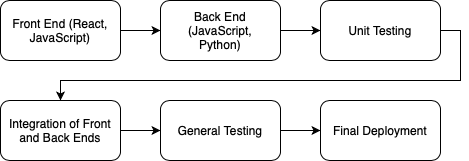
\includegraphics[width=0.95\linewidth]{task.png}
    \end{figure}

\subsection{Migration to the New Product}
\begin{itemize}
    \item Converting the game mechanics from Python to JavaScript
    \item Making the output in an HTML format, rather than a console output
    \item Adding new features available with the web app format
\end{itemize}

\subsection{Risks}
\begin{itemize}
    \item Runner Failure - 1 percent Chance in the event that it happens Reboot service within 12 hours
    \item Communication failure between back-end and front-end, resolve by rebooting the system
\end{itemize}

\subsection{Costs}
So long as free online tutorials and resources are used exclusively, the only costs will pertain to time devoted to developing the product, specifically in weekly meetings.

\subsection{User Documentation and Training}
Documentation of the different functions and files in the product will be provided separately, detailing the purpose of the function, as well as how it operates, what variables it takes in, and what it outputs. 
The users of the product will require no training, as the game will clarify which keys are used in playing the game, and the UI being clear enough for a first-time user to navigate with ease and without confusion.

\subsection{Waiting Room}
Advanced features of the game may not be included in its initial release, possibly including:
\begin{itemize}
    \item 2-player mode
    \item Player customization of the game (i.e different color themes)
\end{itemize}

\subsection{Ideas for Solutions}
\begin{itemize}
    \item Using free online resources to gain a better understanding of JavaScript and React
    \item Constant, clear, and consistent communication between group members on matters of roles, current progress, coding functionality, and coding style, typically through group meetings, GitLab commits, and code commenting/documentation
\end{itemize}

\bibliographystyle{plainnat}

\bibliography{SRS}

\newpage

\section{Appendix}

This section has been added to the Volere template.  This is where you can place
additional information.

\subsection{Symbolic Parameters}

The definition of the requirements will likely call for SYMBOLIC\_CONSTANTS.
Their values are defined in this section for easy maintenance.


\end{document}